\section{Application Overview}
\label{sec:appOver}


\subsection{Users}
Any person, Government officials, or someone in the private sector who wants to read and understand the basic risk profile of their region and make decisions with that information.

\subsection{Architecture}

Figure \ref{fig:archi} shows the architecture of the proposed solution including the elements of the application at component level and its connections at high level (see deployment diagram). Additionally, it shows the application elements used for the Front and Back End. The figure also shows the names of the technologies used hosted on AWS cloud, i.e.: (Python, dash and libraries).   

The following is the list AWS components used in the project: 
\begin{enumerate}
\item The machine who host the solution (Elastic Compute Cloud - EC2). 
\item The Database  (Relational Database Service -RDS).
\item The storage for the datasets and GeoJson files for Colombia on the service  (Simple Storage Service - S3) to save these files.
\item The Security group for these services talks with each other and have access from the internet as well.
\item The remote DNS (Domain Name Service) to have a friendly URL for the application on the Apache Web server.
\item A remote code repository (hosted by github). It is used for hosting the source code and documentation. 

\end{enumerate}


\begin{figure}%
\centering
\subfigure[Deployment diagram]{%
\label{fig:first}%
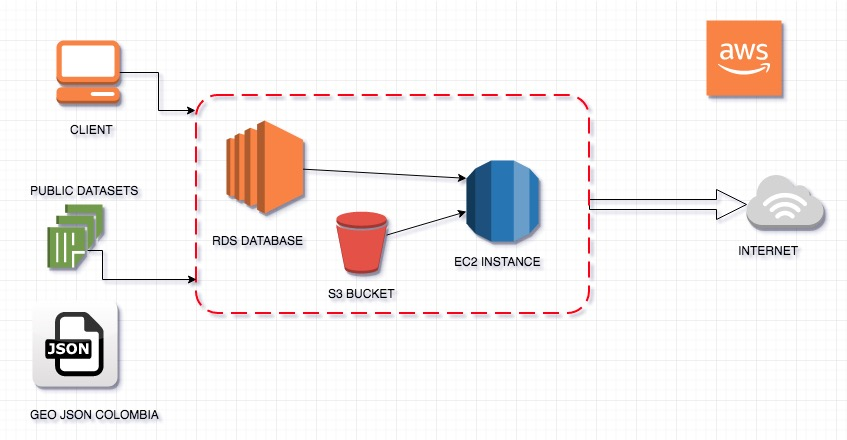
\includegraphics[height=3in, width=4.5in]{../../../aws_diagrams/AWS_Deployment_Diagram_project_group_03}}%
\qquad
\subfigure[Component diagram]{%
\label{fig:second}%
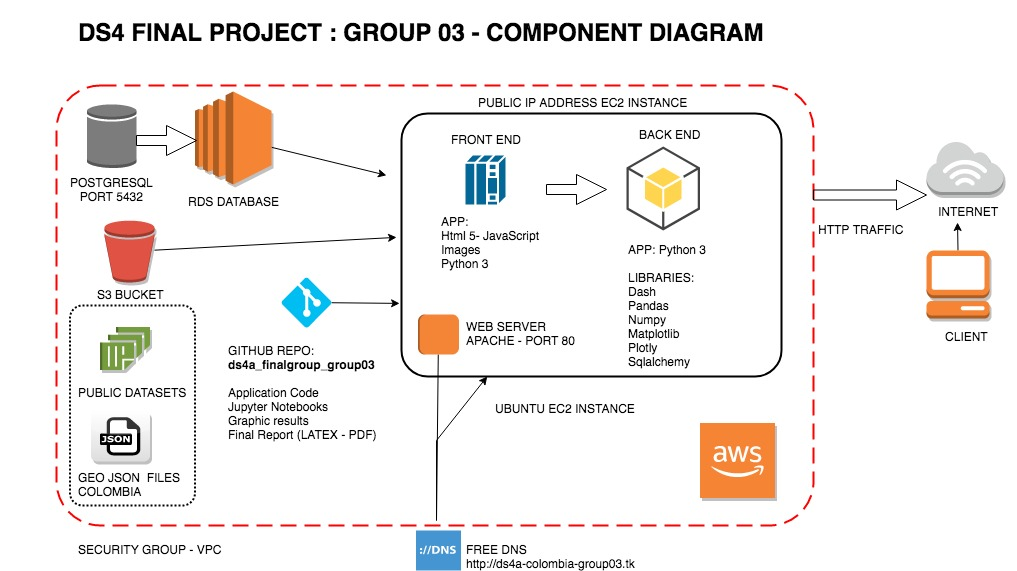
\includegraphics[height=4in, width=6in]{../../../aws_diagrams/AWS_Component_Diagram_project_group_03}}%
\caption{Project architecture.}
\label{fig:archi}%
\end{figure}





\subsection{Front End Design}

The following is the link of the web-page created for the project. \\
 \url{http://ds4a-colombia-group03.tk/}
%\item \href{https://marioceron-case-51.s3.amazonaws.com/final_project/front_end/index.html}{http://ds4a-colombia-group03.tk/} 

In general terms, the proposed information system will provide a dynamic map of Colombia with:

\begin{enumerate}
\item Impact variables such as Deaths, People and Houses affected.
\item A map (Main View) that will show the index adjusted by capacity ( \'Indice Ajustado por Capacidades). By default, the map starts with the country view with political division (departamento).
\item A timeline slider will facilitate the visualization of the index using time intervals. 
\item Considering the established association between extreme temperatures and the frequency of hydro-meteorological events, a projected extreme-temperature indicator for the 100 most vulnerable municipalities with 3 data points: Indicator value at Time 0 (1998), Time 1 (2018) and Time 3 (projected 2040). The indicator corresponds to the extreme temperature projection made by Climate Impact Lab for the number of days a year that register temperatures above 32 degrees Celsius.

\item The option of showing political divisions views (vista de departamento). The user can select the small political subdivision (municipio) and the graphics on the right side of the dashboard screen are updated.
\end{enumerate}




\begin{figure}%
\centering
\subfigure[Presentation page]{%
\label{fig:first}%
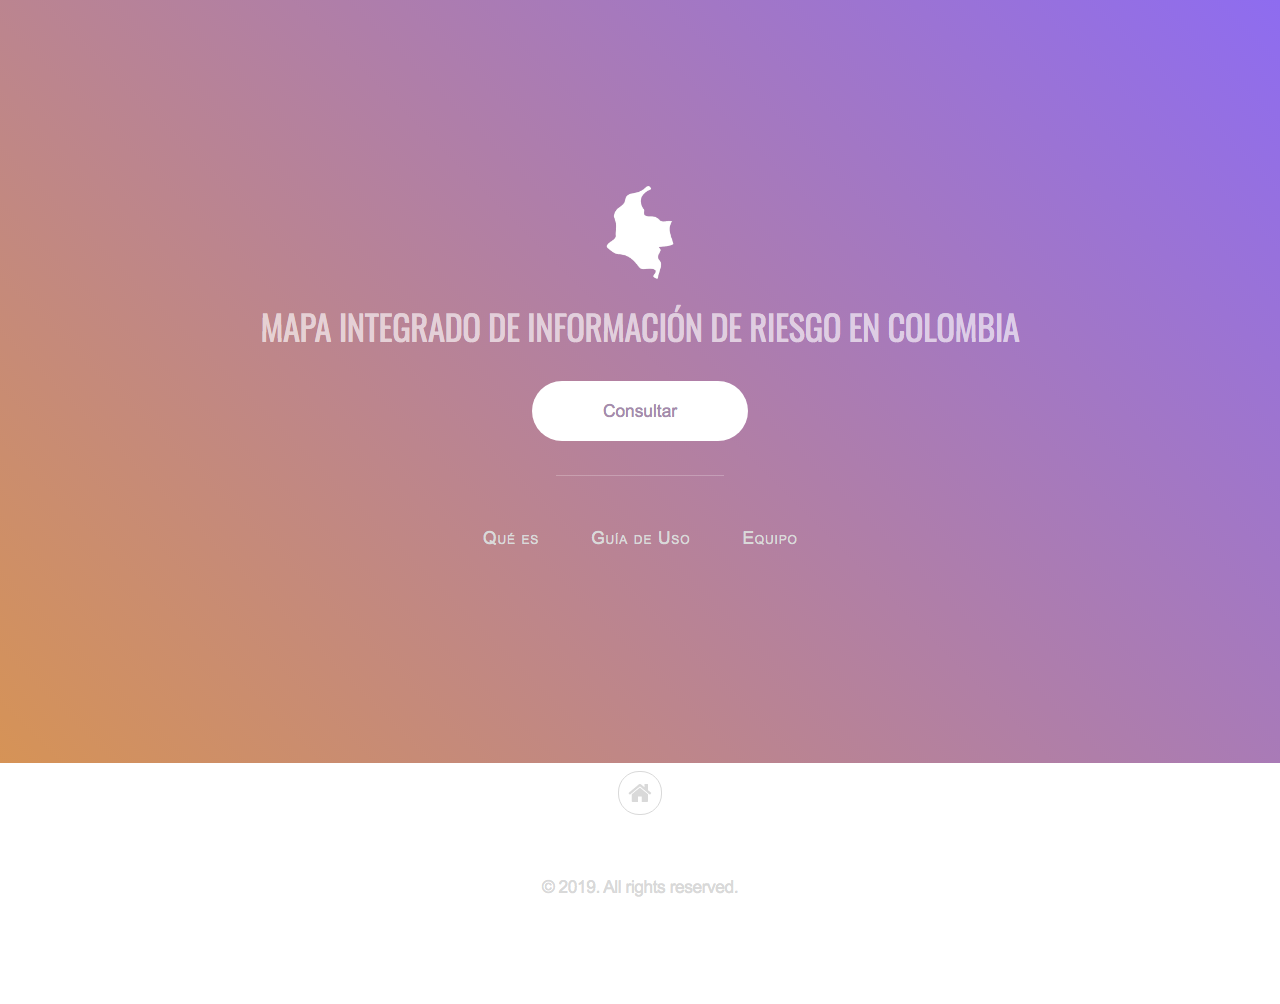
\includegraphics[height=4in, width=6in]{01_Home_ds4a-colombia-group03-tk.png}}%
\qquad
\subfigure[Main page]{%
\label{fig:second}%
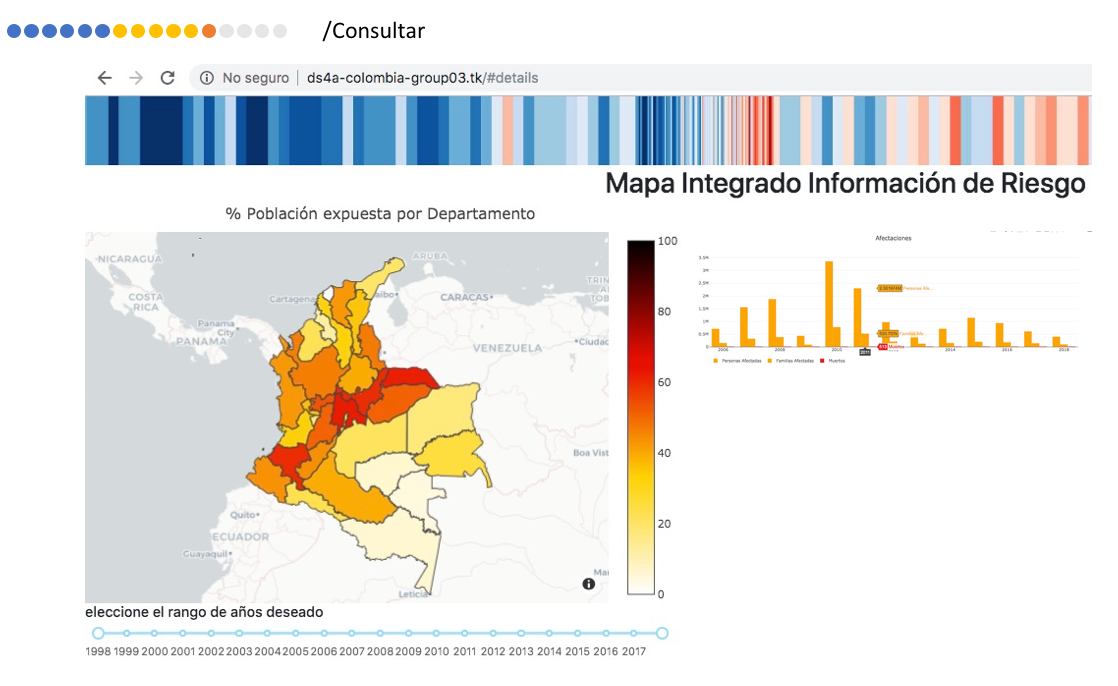
\includegraphics[height=4in, width=6in]{02_Home_mapa.png}}%
%\subfigure[]{%
%\label{fig:second}%
%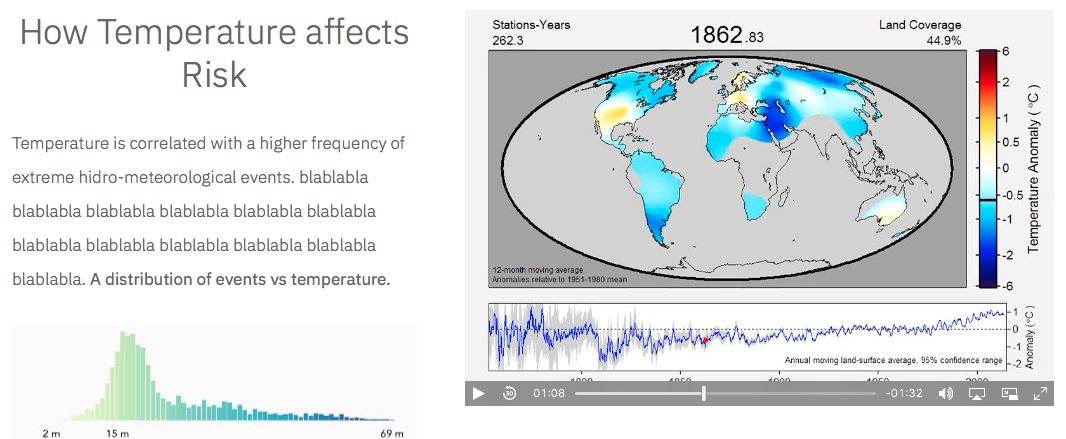
\includegraphics[height=2in, width=3in]{riesgo6}}%
\caption{Front End: Integrated Map of Risk Information in Colombia. The main page (Figure \ref{fig:first}) will show the map of Colombia with the Risk Index, and will offer interactive options to get detail information of selected Municipalities, risk index and a projected temperature indicator.}
\label{fig:muckup}%
\end{figure}

